\documentclass [MAS] {uclathes}

% \input {mymacros}                         % personal LaTeX macros

%%%%%%%%%%%%%%%%%%%%%%%%%%%%%%%%%%%%%%%%%%%%%%%%%%%%%%%%%%%%%%%%%%%%%%
%
% Usually things live in separate flies.
%
% \input {prelim}                           % preliminary page info

%%%%%%%%%%%%%%%%%%%%%%%%%%%%%%%%%%%%%%%%%%%%%%%%%%%%%%%%%%%%%%%%%%%%%%%%
%                                                                      %
%                          PRELIMINARY PAGES                           %
%                                                                      %
%%%%%%%%%%%%%%%%%%%%%%%%%%%%%%%%%%%%%%%%%%%%%%%%%%%%%%%%%%%%%%%%%%%%%%%%

\title          {An Application of Split Attention Networks:\\
                Melanoma Detection}
\author         {Andrew Mashhadi}
\department     {Statistics}
\degreeyear     {2023}

%%%%%%%%%%%%%%%%%%%%%%%%%%%%%%%%%%%%%%%%%%%%%%%%%%%%%%%%%%%%%%%%%%%%%%%%

\chair          {Yingnian\ Wu}
\member         {Frederic Paik\ Schoenberg}
\member         {Michael Tsiang}

%%%%%%%%%%%%%%%%%%%%%%%%%%%%%%%%%%%%%%%%%%%%%%%%%%%%%%%%%%%%%%%%%%%%%%%%

\abstract       {(Abstract temporarily omitted)}

%%%%%%%%%%%%%%%%%%%%%%%%%%%%%%%%%%%%%%%%%%%%%%%%%%%%%%%%%%%%%%%%%%%%%%%%

\usepackage{subcaption} 
\usepackage{graphicx}
\usepackage{amsmath}
\usepackage{amsfonts}
\usepackage{array, makecell}
\renewcommand\cellset{\renewcommand\arraystretch{0.8}%
\setlength\extrarowheight{0pt}}

%%%%%%%%%%%%%%%%%%%%%%%%%%%%%%%%%%%%%%%%%%%%%%%%%%%%%%%%%%%%%%%%%%%%%%%%

\begin {document}

\makeintropages

%%%%%%%%%%%%%%%%%%%%%%%%%%%%%%%%%%%%%%%%%%%%%%%%%%%%%%%%%%%%%%%%%%%%%%%%

\chapter{Introduction}

\section{Background}

In the past decade, machine learning has exploded in popularity. Machine learning methods have demonstrated endless applciations to a variety of industries including but not limited to engineering, science, finance, medicine, and technology. A large branch of machine learning that has recently taken the world by storm is \textit{deep learning}. Deep learning is made up of \textit{artificial neural networks} (ANN) and is generally trained with a form of \textit{feature learning}. 

Neural network architures have evolved and expanded since the original perceptron and ANN models. Through different areas of application, variations in neural network architecture such as \textit{deep neural networks}, \textit{convolutional neural networks}, \textit{recurrent neural networks}, and more recently \textit{transformers}, have all been proposed and adopted. It is no secret that the transformer model has quickly become a front-runner for applications in computer vision due to its successes in natural language processing. However, deep convolutional neural networks are still state-of-the-art for tasks such as image classification, object detection, semantic segmentation, and instance segmentation

Different learning methods have also been adopted. However, the type of learning method used generally depends on the model's particular objective. \textit{Supervised Learning} is one of the most common methods for classification or regression models. It is the process of using labeled datasets to train machine learning models to classify or predict outcomes appropriately. \textit{Unsupervised Learning} generally involves the analysis or clustering of unlabeled datsets. And \textit{Reinforcement Learning} is based on rewarding desired behaviors and/or punishing undesired ones.

More recently, the medical community has been opening it's doors to modern deep learning techniques. In particular, convolutional neural networks (CNNs) have often been used to develop more efficient, and accurate, diagnostic tools to analyze medical images. Due to the growth of effective image recognition models, collection of medical images for specific applciations in the healthcare community have been been growing. 


\section{Problem Statement}

Skin cancer is one of the most common types of cancer. Although melanoma only accounts for about 1\% of skin cancer, the death rate was still about 2.1 per 100,000 men and women per year based on 2016-2020 deaths \cite{SEER}. In 2023, the American Cancer Society estimates that bout 7,990 people are expected to die from a total of about 97,610 new melanoma cases in the United States alone \cite{ACS}. It is well known that early detection of melanoma will provide the best chance for successful treatment and greater chance of survival. 

Image analysis tools that automate the diagnosis of melanoma will improve dermatologist's diagnostic accuracy, and better detection of melanoma has the opportunity to positively impact millions of people. Providing an accurate machine learning model to aid dermatologist's in their evaluations of patients moles may lead to an earlier diagnoses, and could therefore provide the best chance for appropriate intervention. We want to use a new deep convolutional-neural-network architecture that uses patients skin-lesion images along with any other patient-level contextual information to determine which patients are likely to have melanoma skin cancer. In particular, the goal of this paper is to identify the presence of melanoma from images of skin lesions using the novel \textit{ResNeSt} architecture that was designed to apply channel-wise attention on different network branches.


\chapter{Dataset}

\section{ISIC 2020 Challenge Dataset}

For this paper, we used the ``ISIC 2020 Challenge Dataset''. This was the official dataset of the SIIM-ISIC Melanoma Classification Challenge hosted as a Kaggle sponsored competition in the Summer of 2020. It contains over 30,000 dermoscopic images of distinct skin lesions from approximately 2,000 patients. Each image has an associated record of metadata. The metadata includes the corresponding ``beniegn'' or ``malignant'' status, as well as the following patient-level features: 

\begin{itemize}
    \item \textit{patient\_id}: unique patient idenitfier
    \item \textit{sex}: sex of the patient 
    \item \textit{age\_approx}: approximate age of the of the patient
    \item \textit{anatom\_site\_general\_challenge}: the general location of imaged lesion
    \item \textit{diagnosis}: additional details regarding the diagnosis
\end{itemize}

We should note that all associated malignant and benign diagnoses have been confimed using histopathology, expert agreement, or longitudinal follow-up \cite{ISIC}.

The International Skin Imaging Collaboration (ISIC) was responsible for compiling the images from the Hospital Clínic de Barcelona, Medical University of Vienna, Memorial Sloan Kettering Cancer Center, Melanoma Institute Australia, University of Queensland, and the University of Athens Medical School to form this official dataset. The ISIC Archive contains the largest collection of quality-controlled dermoscopic images of skin lesions available to the public. 

The resolution of each image varied drastically throughout the dataset, with some images reaching as high as $4000 \times 6000$ pixels. The set of images consisted of over 110GB, so we hosted the data on UCLA's Hoffman2 Linux Cluster. To support the size of each image and the large number of individual images within the dataset, we used computing resources from the Hoffman2 cluster and Google Colab to tune, train, and test our models with powerful \textit{Graphical Processing Units} (GPUs). Although the GPU would occasionally change, we mostly used a single NVIDIA A100 GPU with approximately 40GB VRAM to train our larger models.

\section{Data Preparation}

Throughout training, we found it to be difficult to train our models without batch-sizes greater than or equal to 16 images. However, computational constraints limited our ability to utilize larger batch-sizes with such large lesion images. We ultimately found that the only way to train efficiently with suffcient batch-size ($B \geq 16$) was to center crop, or resize (using bilinear interpolation), each original lesion image to a fixed-sized $512 \times 512$ image. Further transformations and resizing are discussed in the methodology section.

The patient-level features within the metadata also required minor preprocessing. We created dummy variables with treatment coding (also known as \textit{one-hot encoding}) for the \textit{sex} and \textit{anatom\_site\_general\_challenge} features, while keeping \textit{age\_approx} as a continuous variable.


\section{Exploratory Data Analysis}

In this section, we provide an exploratory data analysis of both the images and the patient-level features within the metadata provided in our dataset.

\subsection{Skin Lesion Images}

The images of skin lesions are the most important part of data for our model. They will be used to train the image classification network, so we decided to investigate the data a bit more, before beginning to model. First, we investigated the proportion of ``positives'' (malignant) and ``negative'' (beniegn) images within our dataset. Table 2.1 presents the balance of malignant and beniegn skin lesions within our dataset. As we can see from the table, there is significantly large class imbalance. Only about 1.8\% of the skin lesion image are classified as malignant. 

\begin{table}[h!]
\centering
\begin{tabular}{| c | c | c |} 
\hline
& Beniegn ($-$) & Malignant ($+$) \\ 
\hline
\hline
Count & 32542 & 584\\
\hline
Proportion & 0.9824 & 0.0176\\
\hline  
\end{tabular}
\label{tab:propMel}
\caption{Proportion of Beniegn \& Malignant Skin Lesions}
\end{table}


As mentioned above, we fixed the resolution of the images in our dataset to 512x512 pixels. We visually inspected the quality of several randomly selected skin lesions images after cropping and resizing to make sure that the \textit{object of interest} (the actually skin lesion itself) was still present and easily distinguishable. In Figures 2.1-2.2 , we present 6 images from our dataset. The top 3 skin lesions were randomly selected from the images flagged as malignant, while the bottom 3 skin lesisons were randomly selected from the images marked as beniegn. Although the relative and absolute size of the skin lesions differ, they are all clearly distinguishable in the images. 

\begin{figure}[hbt!]
\hspace*{\fill}
\centering
\subcaptionbox*{}{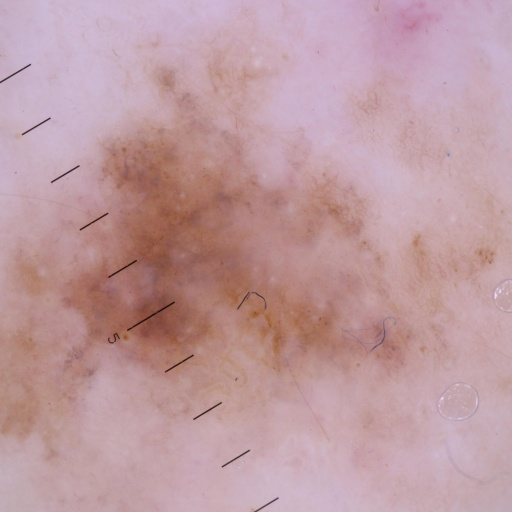
\includegraphics[height = 50mm, width=50mm]{imgs/mal_ex1.jpg}}\hspace{0.5em}
\subcaptionbox*{}{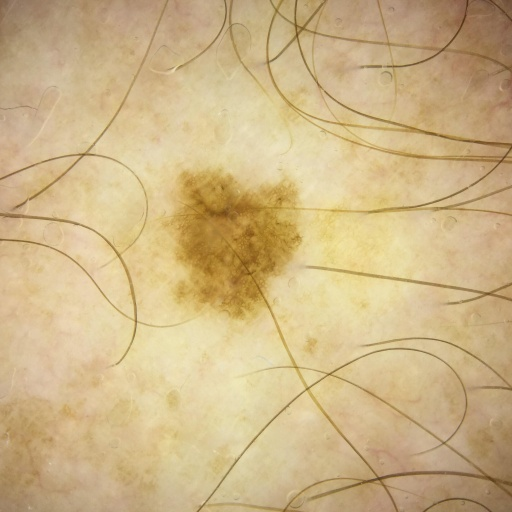
\includegraphics[height = 50mm, width=50mm]{imgs/mal_ex2.jpg}}\hspace{0.5em}
\subcaptionbox*{}{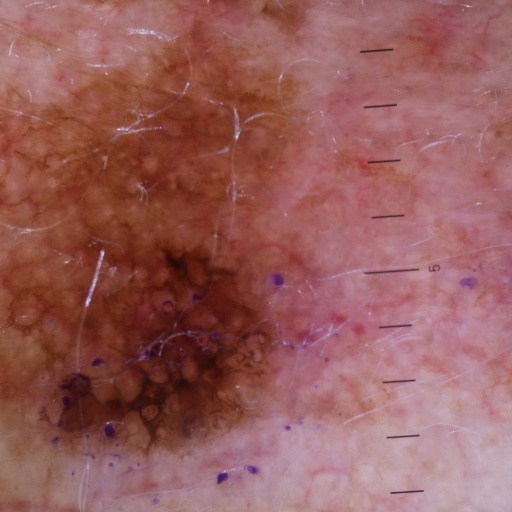
\includegraphics[height = 50mm, width=50mm]{imgs/mal_ex3.jpg}}
\hspace*{\fill}
\label{fig:mel_examples}
\vspace{-1cm}
\caption{Examples of Malignant Skin Lesions}
\end{figure}

\begin{figure}[hbt!]
\hspace*{\fill}
\centering
\subcaptionbox*{}{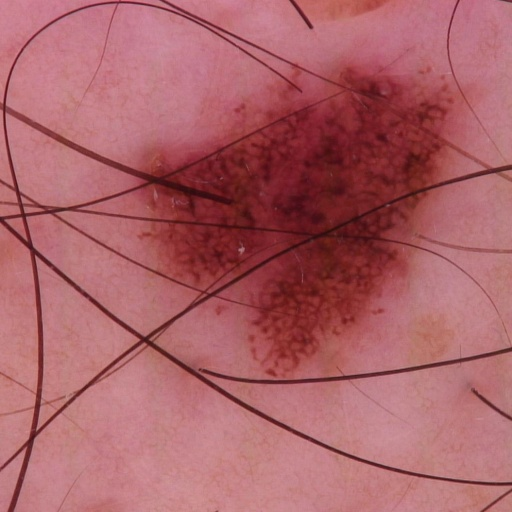
\includegraphics[height = 50mm, width=50mm]{imgs/ben_ex1.jpg}}\hspace{0.5em}
\subcaptionbox*{}{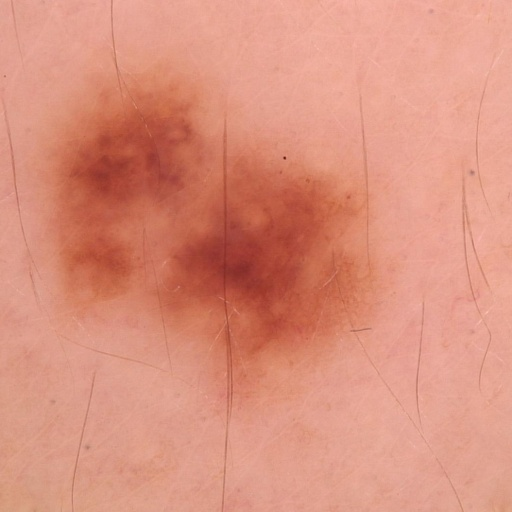
\includegraphics[height = 50mm, width=50mm]{imgs/ben_ex2.jpg}}\hspace{0.5em}
\subcaptionbox*{}{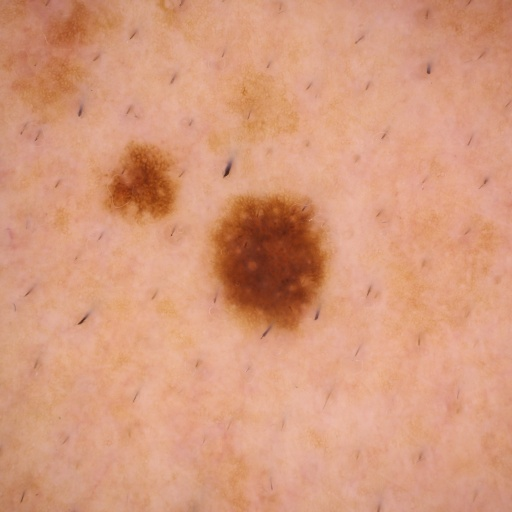
\includegraphics[height = 50mm, width=50mm]{imgs/ben_ex3.jpg}}
\hspace*{\fill}
\label{fig:ben_examples}
\vspace{-1cm}
\caption{Examples of Beniegn Skin Lesions}
\end{figure}


We also visually compared a random collection of images flagged as malignant with another random collection of images flagged as benign. The objective here was to see if our ``untrained'' eye could easily classfiy the skin lessions as malignant or beniegn. We can see from Figures 2.1-2.2 that without proper training and eductaion, it is very difficult to determine whether or not a skin lesion is considered malignant. Even with the proper training, it can still be difficult to accurately determine if melanoma is present. According to the Skin Cancer Foundation, features such as assymmetry shapes, irregular borders, uneven distribution of color, and large relative size may indicate the presence of melanoma (or other skin cancers) \cite{SCF}. Ideally, our network will pick up on these characteristics while training.

\subsection{Patient-Level Features}

In this section we explore the one-way frequency tables for the approximate ages, patient sexes, and the locations of imaged lesions. Then we explored the two-way frequency tables for each of these variables with the response variable (malignant or beniegn).

\subsubsection*{Patient Age}

We can see from the histogram of approximate ages in Figure 2.3(a) that most of the patients in this data are in their 40's, 50's, and 60's. The box-plot in Figure 2.3(b) clearly indicates that older patients are generally associated with a larger number of malignant skin lesions.

\begin{figure}[hbt!]
\hspace*{\fill}
\centering
\subcaptionbox{}{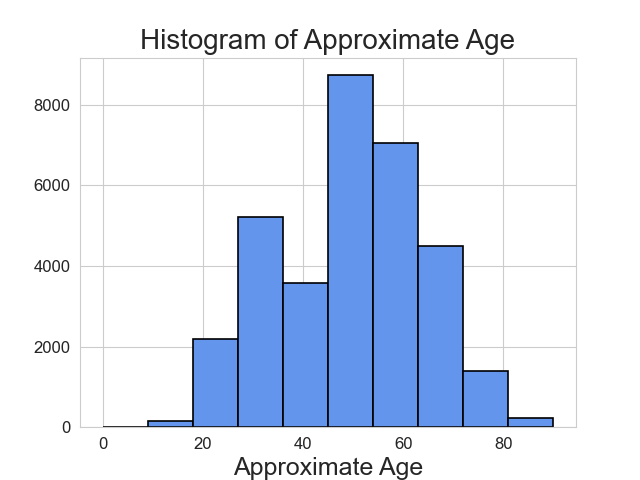
\includegraphics[height = 60mm, width=80mm]{imgs/age.png}}\hspace{0.5em}
\subcaptionbox{}{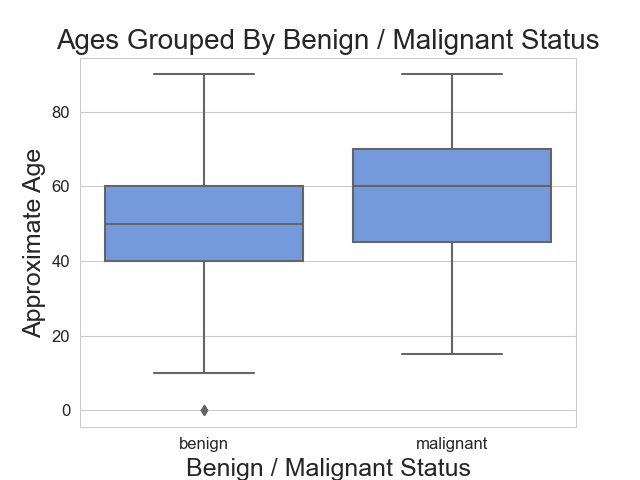
\includegraphics[height = 60mm, width=80mm]{imgs/age_2way.png}}
\hspace*{\fill}
\label{fig:age_eda}
\vspace{0cm}
\caption{Histogram and Box-Plot For Appoximate Age}
\end{figure}

\subsubsection*{Patient Sex}

We can see from the frequencies shown in Figure 2.4(a) that there are a similar number of males and females in this dataset, with just one or two thousand more males. The two-way contingency table between the response variable and patient sex is also shown in Figure 2.4(b). We can see that the malignant cases have a significantly larger proportion of males than the beniegn cases do. In fact, the $\chi^2$-test of independence reported a p-value very close to 0. Therefore, we reject the hypothesis that patient sex and the presence of melanoma are independent, and conclude that there is a relationship between the two variables.

\begin{figure}[h!tbp]
    \hspace*{\fill}
    \centering
    \subcaptionbox{}{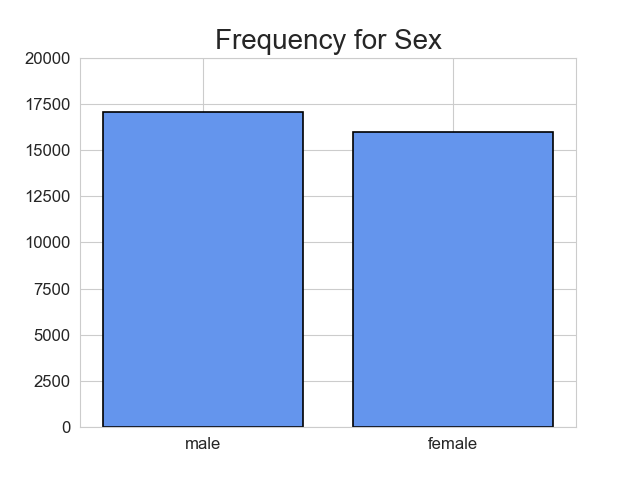
\includegraphics[height = 60mm, width=80mm]{imgs/sex.png}}\hspace{1em}
    \subcaptionbox{}{\vspace{17mm} \footnotesize \begin{tabular}{| c || c | c |} 
        \hline
        & \textbf{Beniegn} & \textbf{Malignant} \\ 
        \hline
        \hline
        \textbf{Female} & 15761 & 220\\
        \hline
        \textbf{Male} & 16716 & 364\\
        \hline  
        \end{tabular}}
    \hspace*{\fill}
    \label{fig:sex_eda}
    \vspace{0cm}
    \caption{Frequency Plot and Two-way Contingency Table for Patient Sex}
    \end{figure}

\subsubsection*{Skin-Lesion Location}

There were 6 categories for the general skin-lesion location: oral/genital, palms/soles, head/neck, upper extremity, lower extremity, and torso. Figure 2.5(a) presents the associated frequencies within our dataset. None of the general locations have a similar number of counts, and almost half of the skin-lesions come from the torso region. We also present the two-way contingency table between the response variable and lesion location in Figure 2.5(b). While it is somewhat difficult to tell, the does appear to be some differences in the balance between beniegn and malignant cases when conditioned on the skin-lesion location. In this case, the $\chi^2$-test of independence also reported a p-value very close to 0, indicating that there is a relationship between the location of the skin-lesion and the presence of melanoma.

\begin{figure}[h!tbp]
    \hspace*{\fill}
    \centering
    \subcaptionbox{}{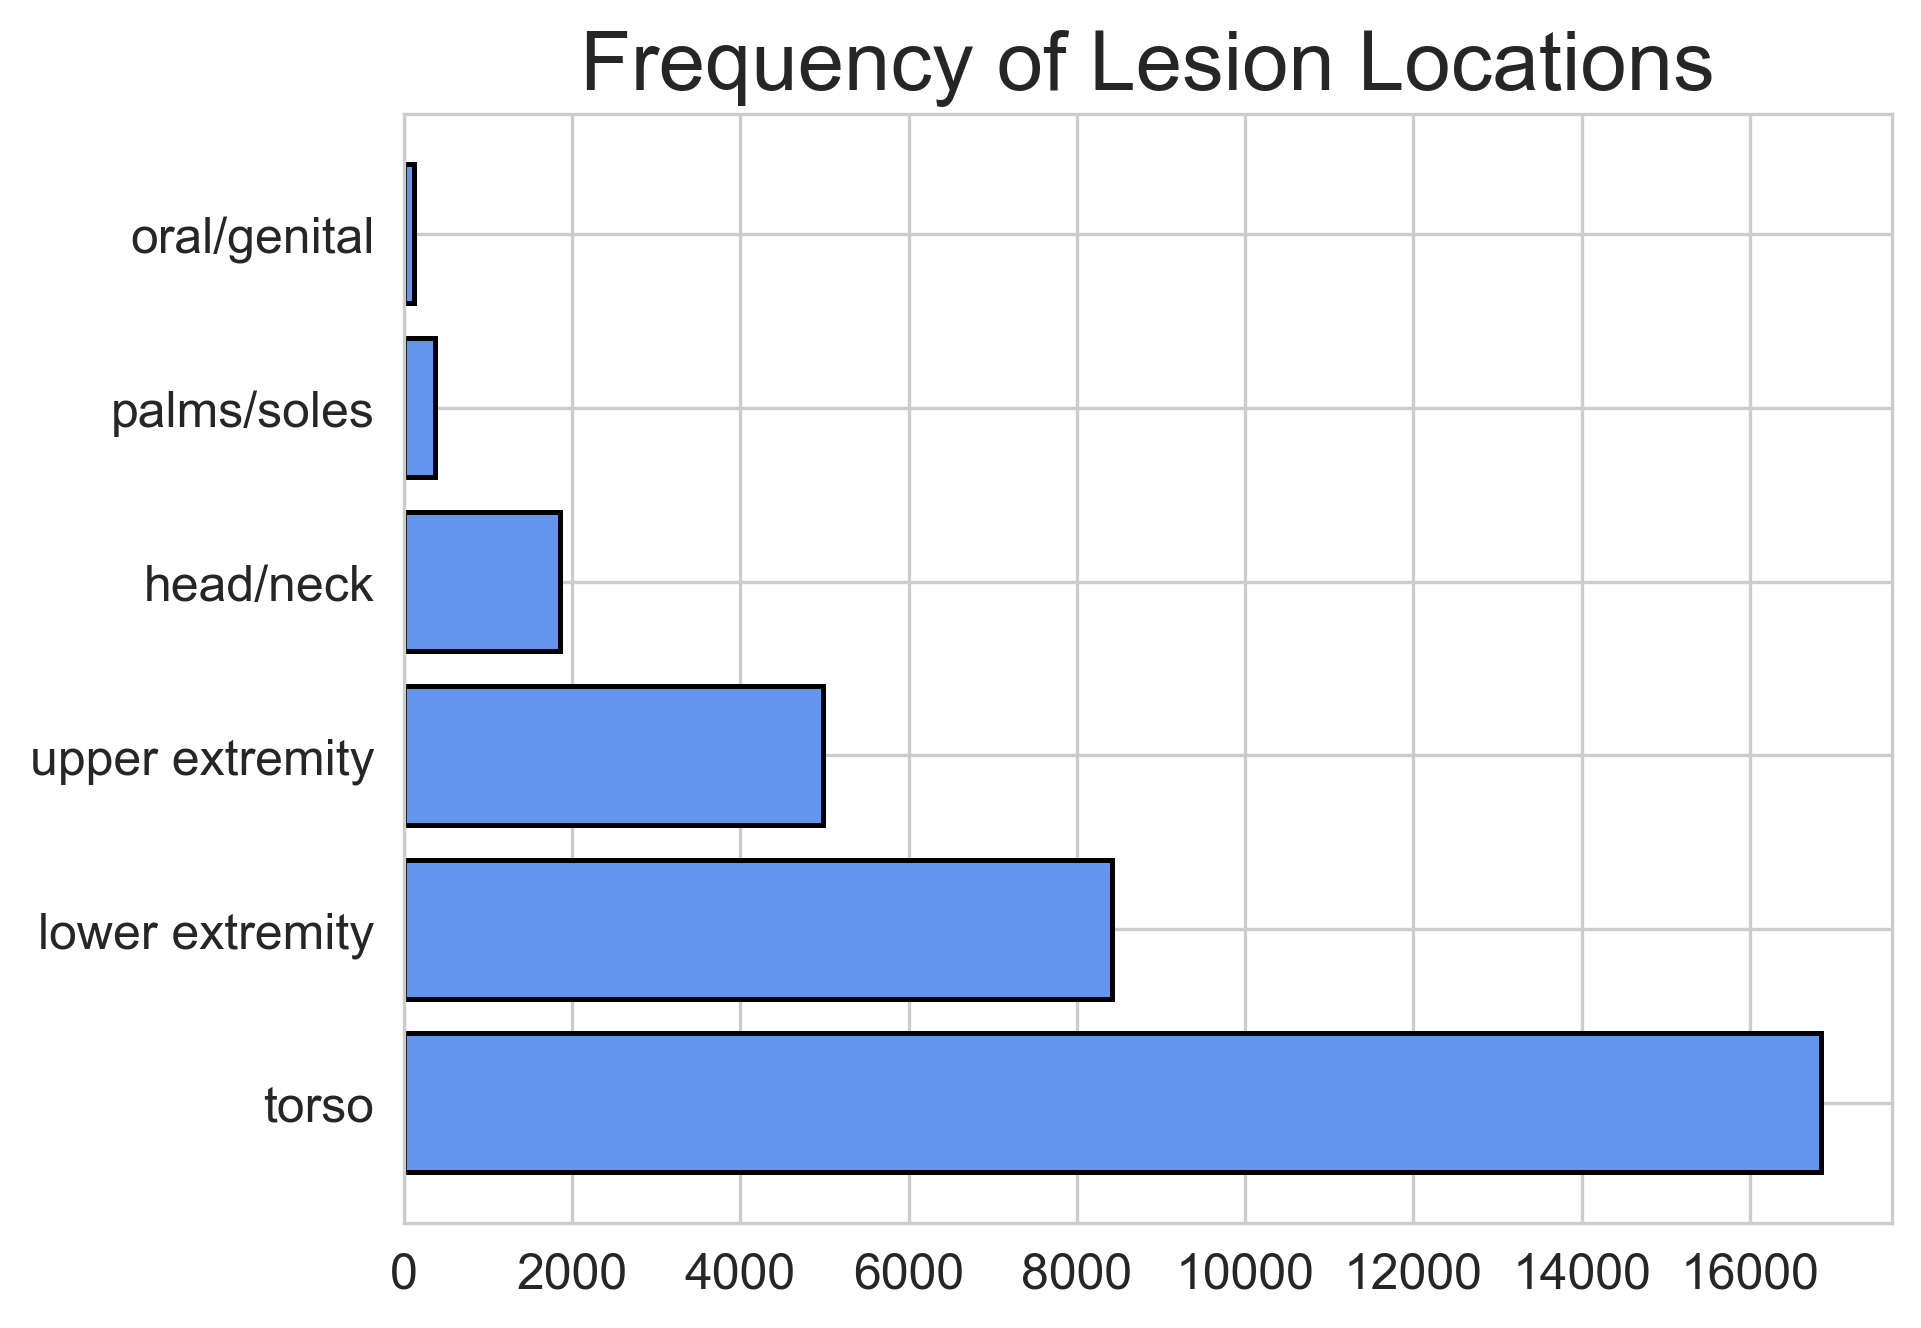
\includegraphics[height = 60mm, width=80mm]{imgs/site.png}}\hspace{1em}
    \subcaptionbox{}{\vspace{5mm} \footnotesize \begin{tabular}{| c || c | c |} 
        \hline
        & \textbf{Beniegn} & \textbf{Malignant} \\ 
        \hline
        \hline
        \textbf{Head/Neck} & 1781 & 74\\
        \hline
        \textbf{Lower Extremity} & 8293 & 124\\
        \hline  
        \textbf{Oral/Genital} & 120 & 4\\
        \hline
        \textbf{Palms/Soles} & 370 & 5\\
        \hline  
        \textbf{Torso} & 16588 & 257\\
        \hline
        \textbf{Upper Extremity} & 4872 & 111\\
        \hline  
        \end{tabular}}
    \hspace*{\fill}
    \label{fig:sex_eda}
    \vspace{0cm}
    \caption{Frequency Plot and Two-way Contingency Table for Lesion Location}
    \end{figure}


\chapter{Methodology}

In this section, we describe the methods and models used to best predict the presence of melanoma. As mentioned above, we used deep convolutional neural networks to generate classifications. More specifically, the latest variant of the residual network, the \textit{ResNeSt}, was used to assess whether or not its channel-wise attention architecture would find further success in melanoma detection. Additionally, we trained a smaller, more traditional, convolutional neural network to compare the performance with the split-attention network. 

To make use of the additional metadata features within our dataset, we simultaneously trained a standard \textit{multi-layer perceptron} (MLP) with inputs from our patient-level features. Therefore, the deep convolutional networks is used to effectively extract any contextualized features from the skin-lesion images and the multi-layer perceptron is used to extract any important patient-level information. The two networks are then connected with eachother before generating a final probability. Since the outputted probabilities are a result from two seperate networks communicating with eachother, this model may be described as a \textit{Multi-Network Ensemble}.

\section{Training, Validation, and Testing Sets}

Before discussing the actual models used, we breifly discuss the how the dataset was split and sampled for training, validating, and testing.

We first randomly split 80\% of the data into a training set and used the other random 20\% as the test set. The test set was
not used by any network during the training process. Additionally, we partitioned another 20\% of the training data into a validation set. Recall that our dataset is largely imbalanced. As shown in the Exploratory Data Analysis section, only about 2\% of the skin lesions in the dataset are flagged as malignant, while the remaining skin lesions are marked as benign. We ensured that each split of the data had a similar sample proportional of about 2\% malignant skin lesions.

Since the response variable (malignant or beniegn) in the training data is heavily imbalanced, we used randomized oversampling of the malignant observations to combat any potential bias toward a ``beniegn'' classification. By oversampling, we hoped that the networks would better detect when skin lesions were truly malignant. It's important to note that since oversampling was used, we considered a single epoch as when the entire \textit{oversampled} dataset was passed forward and backward through the network exactly once. Therefore, a single epoch will contain multiple repeated malignant skin lesion images.

Note that using standard $k$-fold cross validation would require a model to be trained $k$ times for each set of hyper-parameters. Given the size of our data and our models, the time it would take to perform this procedure was simply infeasible. Therefore, we used the independent validation set to tune each network's hyper-parameters effectively. This method minimized overall training time, and produced optimal hyper-parameters. Once the hyper-parameters were obtained, we retrained the model on a new oversampled dataset made up from combining the training and validation sets.

We tuned each model with the area under the \textit{Receiver Operating Characteristic} (ROC-AUC) as our performance
metric. The ROC-AUC was chosen over other metrics because it summarizes how well our network separates the two response
classes over \textit{all} possible thresholds (as opposed to a single predetermined threshold). 

\section{Image Augmentations}

\textit{Image augmentations} were used as a preprocessing step for each image before training. Some image augmention methods are often used to alter the original images in the dataset to effectively create more ``unseen'' examples for the network to use while training. These techniques artificially extends the dataset by randomly providing alerations to existing data, and consequently reduces the chance of overfitting. Given the limited number of malignant examples, this technique is very important to artificially extend our malignant skin-lesion training images. In our networks, we randomly employed the following image augmentations (in this order) on our training data \cite{AUG}:

\begin{enumerate}
    \item \textbf{HueSaturationValue}: With probability $p=0.5$, we randomly changed the hue, saturation, and value of the input image. The shift in hue was between $(-5, 5)$, the shift in saturaion was between $(-10, 10)$, and the shift in value was between $(-5, 5)$.
    \item \textbf{FancyPCA}: With probability $p=0.2$, perform \textit{principal component analysis} on the set of RGB pixel values throughout the imput image, then add multiples of the found principal components, with magnitudes proportional to the corresponding eigenvalues times a random variable drawn from $\alpha_1, \alpha_2, \alpha_3 \stackrel{i.i.d}{\sim} \mathcal{N}(0, 0.1)$.
    \item \textbf{VerticalFlip}: With probability $p=0.5$, we veritially flipped the imput image. Note that vertically flipping the image should not change the true class of the skin lesion.
    \item \textbf{HorizontalFlip}: With probability $p=0.5$, we veritially flipped the imput image. Note that vertically flipping the image should not change the true class of the skin lesion.
    \item \textbf{GaussNoise}: we applied gaussian noise to the input image. We did not want to corrupt the image too much and to ooften, so we used a mean of $0$ and a variance between $(10, 50)$ with a low probability $p=0.2$.
    \item \textbf{ShiftScaleRotate}: With probability $p=0.5$, we randomly applied the three affine transforms: translate, scale and rotate the input. The shift factor range for both height and width was set to $(-0.25, 0.25)$, the scaling factor range was set to $(-0.25, 0.25)$, and the rotation range was set from $-30$ degrees to $30$ degrees. 
    \item \textbf{RandomBrightnessContrast}: With probability $p=0.5$, we randomly modified the brightness and contrast of the input image. Since many of the images were already very dark, the factor range for changing brightness was set to $(0.9, 1.1)$. The factor range for changing contrast was also set to $(0.9, 1.1)$.
\end{enumerate}

Some image augmentations techniques are also used to make sure the images in the dataset work with our models, and may promote faster convergence. For instance, in addition to the above augmentations, we also randomly cropped each $512 \times 512$ image to a 416x416 image and normalized the pixel values to have a similar distribution. Although the randomness of the cropping does somewhat ``artificially'' extend our training set, the main point of cropping the images to $416 \times 416$ is because the ResNeSt network we used requires an input size of $416 \times 416$ pixels. The normalization of the pixel values will reduce the risk of exploding gradients, which has been shown to increase training time and generally slows down convergence. We normalized each channel using the associated sample means and sample standard deviations calculcated from the \textit{ImageNet} database. The ImageNet database consists of millions of images and was designed for use in visual object recognition software research. Although we could have used the sample means and sample standard deviations from our own dataset, using the sample statistics from the ImageNet database is common practice and was recommended by the authors of the \textit{ResNeSt} network.

We should note that most of the above image augmentations were only used on the training set. The validation and testing sets only center cropped the images to $416 \times 416$ and normalized the pixels to work with the trained network.

\section{Network Architectures \& Training}

In the section, we provide an overview of the foundational neural network architectures and we breifly discuss how our networks were trained. We also introduce a few of the techniques we employed to combat overfittins.

\subsection{Multi-Layer Perceptrons}

As illustrated in Figure 3.1, a standard multi-layer perceptron (MLP) model consists of an input layer and an output layer, with at least one hidden layer in between. 


\begin{figure}[h]
\centering
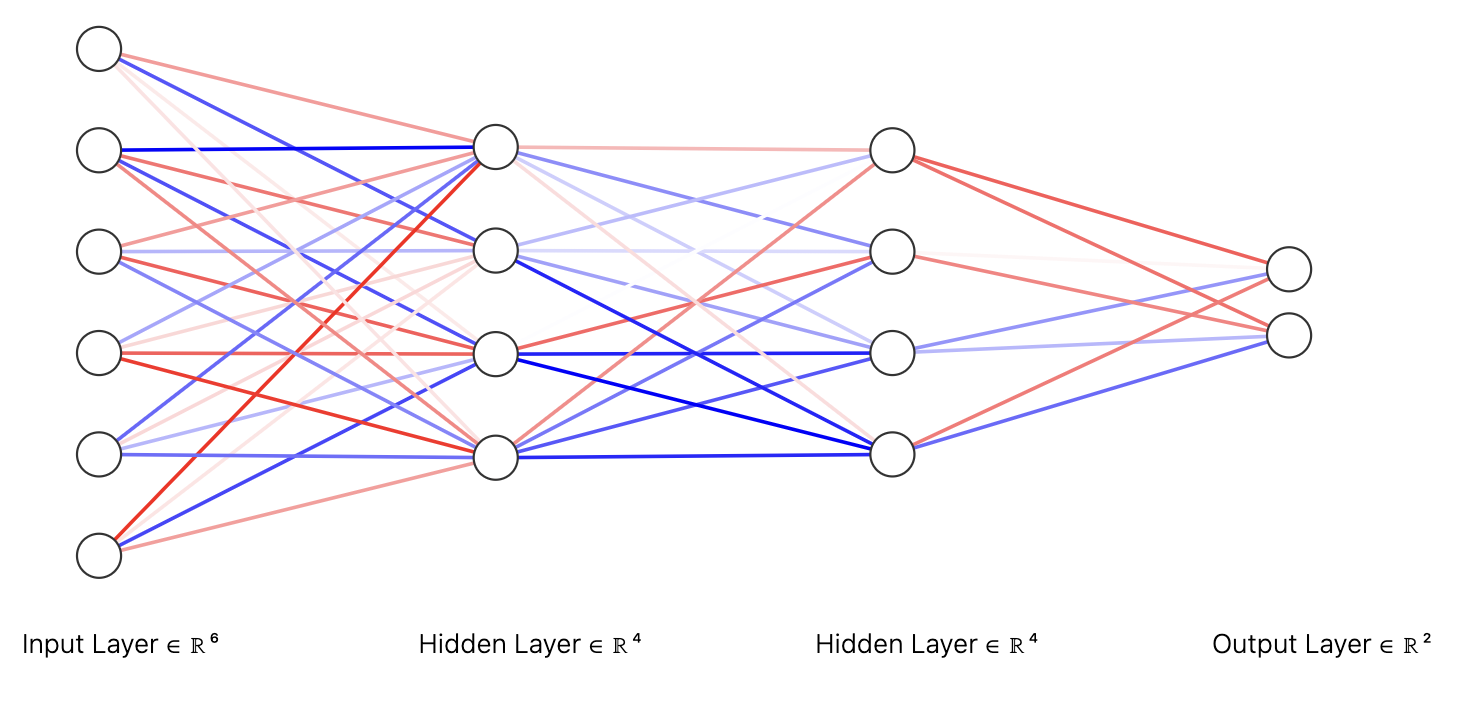
\includegraphics[height = 80mm, width=130mm]{imgs/ffn.png}
\caption{A Standard Feed-Forward Network}
\label{fig:ffn}
\end{figure}

The $l$th layer within the network may be represented by a vector, $\mathbf{h}^{(l)}$, which is obtained by applying a Sigmoid or ReLU transform to the product of the $(l-1)$th layer and a weight matrix, $\mathbf{W}^{(l)}$, plus a bias vector, $\mathbf{b}^{(l)}$. That is, the general MLP has the following recursive structure, $$\mathbf{h}^{(l)} = f_l(\mathbf{s}^{(l)})$$
$$\mathbf{s}^{(l)} = \mathbf{W}^{(l)}\mathbf{h}^{(l-1)} + \mathbf{b}^{(l)}$$ for $l=1, 2, ..., L$. Here, $L$ is the number of layers in the network, $\mathbf{h}^{(0)}$ represents our input features $\mathbf{X}$, $\mathbf{h}^{(K)}$ represents the outputted probabilites used to make the final calssification for our response, $\mathbf{Y}$, and $f_l$ is an element-wise transformation. Following industry standards, our networks used the ReLU activation function for all hidden layers such that $f_l(s^{(l)}_j) = \text{ReLU}(s^{(l)}_j) = \max(0, s^{(l)}_j)$ for $l=1, 2, ..., L-1$ and the softmax function (or sigmoid function if $s^{(K)} \in \mathbb{R}$) for the output layer transformation such that the $j$th outputted probability is:

$$\hat{p}(\mathbf{X})_j = f_K(\mathbf{s}^{(L)})_j = \frac{e^{s^{(L)}_j}}{\sum_i e^{s^{(L)}_i}} \in (0, 1)$$

\subsection{Methods of Learning}

In general, neural networks are trained by minimizing a chosen loss function $L$, with some form of gradient descent. The gradients for each layer's weights $\mathbf{W}_l$ and bias $\mathbf{b}_l$ are calculated using \textit{back-propogation}. Back-propogation is essentially the process of applying chain rule as many times as necessary to obtain the gradient for a specified weight or bias. Given the network structure described above, the following relationships between gradients can be easily shown with chain rule:
$$\frac{\partial L}{\partial \mathbf{h}^{(l-1) \text{ }T}} = \frac{\partial L}{\partial \mathbf{h}^{(l) \text{ }T}} f'_{l} \mathbf{W}^{(l)} \text{,\quad \quad} \frac{\partial L}{\partial \mathbf{W}^{(l)}} = f'_{l} \frac{\partial L}{\partial \mathbf{h}^{(l)}}\mathbf{h}^{(l-1) \text{ }T} \text{,\quad \quad} \frac{\partial L}{\partial \mathbf{b}^{(l)}} = f'_{l} \frac{\partial L}{\partial \mathbf{h}^{(l)}}$$ where $f'_{l} = \text{diag}(f'(s^{(l)}_{j})  \text{; for } j = 1, 2, ... d)$.


For notational convenience, we can represent our training data as $(\mathbf{x}_i, y_i)$ for $i = 1, 2, ..., N$ and our network parameters as $\theta = (\mathbf{W}_l, \mathbf{b}_l  \text{; for } l = 1, 2, ... d)$. Since we have a binary response variable (the skin lesion is either malignant or beniegn), we trained our networks using the \textit{Binary Cross-Entropy} loss function defined as: 

$$L(y_i, \mathbf{x}_i; \theta) = - \left[ y_i\log(\hat{p}(\mathbf{x}_i)) + (1 - y_i)\log(1 - \hat{p}(\mathbf{x}_i)) \right]$$ 

As mentioned above, this loss function is used to train the network's parameters with a form of gradient descent. With $\mathcal{L}(\theta) = \frac{1}{N} \sum_{i=1}^{N} L(y_i, \mathbf{x}_i; \theta)$ as the averaged loss over the entire training set, the standard gradient descent algorithm has the following form: $$\theta_{t+1} = \theta_{t} - \eta_t \mathcal{L}'(\theta_t)$$ where $\mathcal{L}'(\theta_t)$ is the gradient and $\eta_t$ is the learning rate ($\eta_t \propto \frac{1}{t}$). The general idea of this algorithm is to pass the training data through the network (known as the \textit{forward pass}), use these predictions with the loss function to calculate the resulting gradients (known as the \textit{back-propagation pass}), then use these gradients to update the parameterss as shown above. Ideally, we find this algorithm finds the weights and biases $\theta$ that minimizes the binary cross-entropy loss function. 

Practically speaking, computing $\mathcal{L}'(\theta_t) = \frac{1}{N} \sum_{i=1}^{N} L'(y_i, \mathbf{x}_i; \theta_t)$ would be far too time consuming with massive traning set and large number of parameters. Instead, we use a randomly selected mini-batch of size $m$ to replace $\mathcal{L}(\theta_t)$ with its estimate: $$\hat{L}(\theta_t) = \frac{1}{m} \sum_{j=1}^{m} L(y_j, \mathbf{x}_j; \theta_t)$$ when updating the parameters. This replacement is known as \textit{Stochastic-Gradient Descent}. This reduces the computation cost at each iteration, and will ideally lead to similar results (assuming a true randomly sampled batch and a large enough $m$). One \textit{Epoch} occurs after the entire training set has been passed though the network exactly once. Therefore, with stochastic gradient descent, a single epoch occurs after about $t=\frac{N}{m}$ updates to the network paramters.

At each iteration, the stochastic gradient descent algorithm described above will always update the parameters in the direction of the steepest darnward direction. This direction may not always be the ideal choice. Depending on the level of noise and the loss function itself, it may be valuable to consider characteristics such as the momentum of the movement and the unevenness of the individual parameter components. The \textit{Adam} optimizer modifies the stochastic gradient descent algoithm by considering the direction of the momentum and includes an adaptive mechanism to reduce the effects of extremely uneven gradient components. At the $t$th iteration, momentum is characterized by: $$\nu_t = \frac{1}{(1-\gamma)} \left[ \gamma \nu_{t-1} + (1-\gamma)\hat{L}(\theta_t) \right]$$ and the mechanism for adjusting the uneven components is: $$G_t = \frac{1}{(1-\beta)} \left[ \beta G_{t-1} + (1-\beta)\hat{L}(\theta_t) \odot \hat{L}(\theta_t)\right]$$ where $\gamma, \beta \in \mathbb{R}$ are tunable hyperparameters. However, they are usually set between $\gamma, \beta \in (0.9, 1)$. 

Consequently, the network parameters are now updated such that: $$\theta_{t+1} = \theta_{t} - \eta_t \frac{\nu_t}{\sqrt{G_t + \varepsilon}}$$ Here $\varepsilon>0$ is a very small constant to avoid division by 0. Note that the generall structure of the parameter update still remains similar to stochasic gradient descent, however, each update also considers the momentum from the previous updates and the variation in the gradient components.

Our melanoma detection networks were trained using this Adam optimizer with $\gamma$ and $\beta$ fixed at $0.9$ and $0.999$, respectively. Throughout training, the initial learning rate $\eta_t$ was tuned using our validation set, however, we customized our networks to tune different learning rates for different branches of our network. That is, the weights and biases from the convolutional network in our ensemble had a \textit{seperately tuned} learning rate from the rest of our ensemble network. This is discussed in more detail in section X.X.X. Additionally, all learning rates were scheduled to decay by a multiplicative factor of $0.1$ after each epoch.

\subsection{Preventing Overfitting}

Given the large number of parameters, neural networks will often overfit the training data if precations are not taken. Overfitting occurs when the network effectively fits the random noise within the data, and lacks the ability to generalize on unseen data. Figure 3.2 shows the general trend of the training vs validation loss as we train our network. The idea is that if we train our model too long, it will overfit the training data, and the predictive performance will be suboptimal for the validation (or test) dataset. 

\begin{figure}[h]
\centering
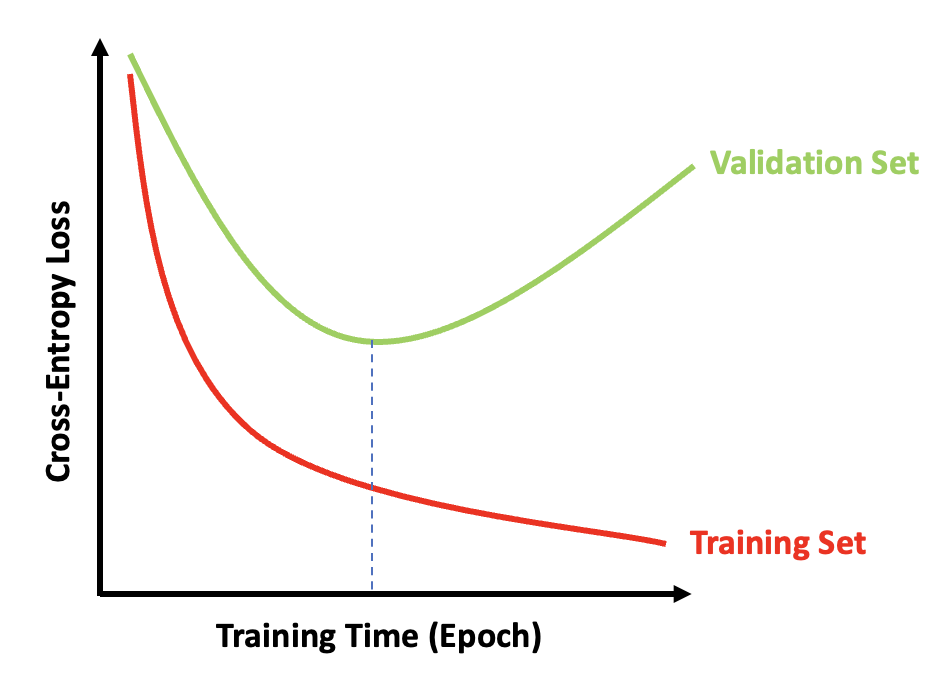
\includegraphics[height = 75mm, width=110mm]{imgs/overfitting.png}
\caption{Overfitting Illustration}
\label{fig:ovfit}
\end{figure}

To prevent our networks from overfitting the training data, we used the validation set to obtain performance updates throughout training, and stoped the training once the validation performance appears to decline. The goal would be to use the parameters that correspond to the minimum validation loss, or maximum validation performance. The vertical dotted line in Figure 3.2 indictes this ideal stopping point. 

In our case, we generated a validation performance update after each half-epoch of training. At each half-epoch, we calculated the ROC-AUC score and the binary cross-entropy loss for the valdiation data, and discontinued the training if these scores dropped or stayed the same in back-to-back performance updates.

There are other methods to help prevent overfitting from occuring. As mentioned above, image augmentation helps prevent the chances of overfitting by artifically increasing size of the training set. We also used \textit{L2-Regularization} for our network parameters. This form of regularization within neural networks is also referred to as \textit{weight-decay}. In general, L2-regularization adds a penalty term, $J(\theta)$, to our loss function such that we want to minimize $\mathcal{L}(\theta) + \lambda J(\theta)$ where: $$J(\theta) = \sum_{l, j, k} {W^{(l)}_{j, k}}^2 + \sum_{l, k} {b^{(l)}_{k}}^2$$ and $\lambda > 0$ is a hyperparameter that we tune while training \cite{ESL}. 

In addition to regularization, we also included \textit{dropout} layers to prevent overfitting. Dropout layers refer to the dropping of a random selection of nodes within a specified layer of the network. All of the connections associated with a dropped node are consequently removed, and the ``new'' network is made up of a subset of original nodes and connections. Dropout can be thought of as another form of regularization because it effectively prevents neurons in a layer from heavily depending on one input. Preventing the overreliance of a single input will reduce the variance of the network parameters. 

Dropout regularization was frequently used throughout our network ensemble with $p = 0.2$. Meaning that a random 20\% of the layer's corresponding neurons were masked while training. 


\subsection{Batch Normalization}

When training the neural network with back-propagation, the distribution of each layer's inputs, $\mathbf{h}^{(l)}$ for $l=1, 2, ..., L$, may often change because the parameters of previous layers ($< l$) are also changing with every mini-batch update. This phenomenon is known as \textit{internal covariate shift}, and it has been shown to drastically slow training time down \cite{BatchNorm}. In our networks, we stabilize the distributions of each layer's inputs, $\mathbf{h}^{(l)}$ for $l=1, 2, ..., L$, using \textit{batch normalization} \cite{BatchNorm}. Therefore, between $\mathbf h^{(l)}$ and $\mathbf h^{(l+1)}$, we added a batch normalization layer that transformed $\mathbf{h}^{(l)}$ to $\tilde{\mathbf{h}}^{(l)}$ to help stabilize its distribution and reduce the internal covariate shift. Then $\tilde{\mathbf{h}}^{(l)}$ is fed into the next layer for the computation of $\mathbf{h}^{(l+1)}$. 

More formally, consider a mini-batch size of $m$, and a layer input $\mathbf{h}^{(l)} = (h^{(l)}_1, ..., h^{(l)}_d) \in \mathbb{R}^d$. Batch-normalization is applied to each element of $\mathbf{h}^{(l)}$ independently, so for each $k \in \{1, 2, ..., d \}$, we have exactly $m$ values of this activation from the mini-batch. For simplicity, we denote the $i$th value from the $k$th activation by $x_{i,k}$ for $i \in \{1, 2, ..., m \}$ and $k \in \{1, 2, ..., d \}$. The batch normalization layer computes $$\mu_k = \sum_{i=1}^{m} x_{i, k} \text{, \quad} \sigma_k = \frac{1}{m} \sum_{i=1}^{m} (x_{i, k} - \mu_k)^2 \text{, \quad} \hat{x}_{i,k} = \frac{x_{i,k} - \mu_k}{\sigma_k} \text{, \quad} y_{i, k} = \beta + \gamma \hat{x}_{i,k}$$ where $\beta$ and $\gamma$ are learned while training. Here, $y_{i, k}$ represents the $i$th value (from the mini-batch) for the $k$th activation of the batch-normalized, layer inputs $\tilde{\mathbf{h}}^{(l)}$, where $i \in \{1, 2, ..., m \}$ and $k \in \{1, 2, ..., d \}$.

These batch-normalization transformations were used after most of the convolutional and linear layers within our ensemble of networks. Although no tuning was necessary for this technique, we found that the inclusion of batch-normalization layers significantly sped up training time.


\subsection{Convolutional Neural Networks}

The convolutional neural network (CNN) structure is often used for computer vision objectives. In general, a CNN is made up by a series of convolutional layers that filter down the training images to a single ``thought'' vector. This ``thought'' vector is a larger linear layer with many nodes/elements that represents extracted features from the images. The final ``thought'' vector is then followed by a series of fully-connected linear layers as if it were a standard multi-layer perceptron. We can think of the ``thought'' vector as a characterization of its associated image. Figure 3.3 illustrates the general idea. Through a variety of transformations and subsampling (or pooling) techniques, the original image is filtered down into a longer, linear, layer that is ultimately used as input for another feed-forward network.

\begin{figure}[h]
\centering
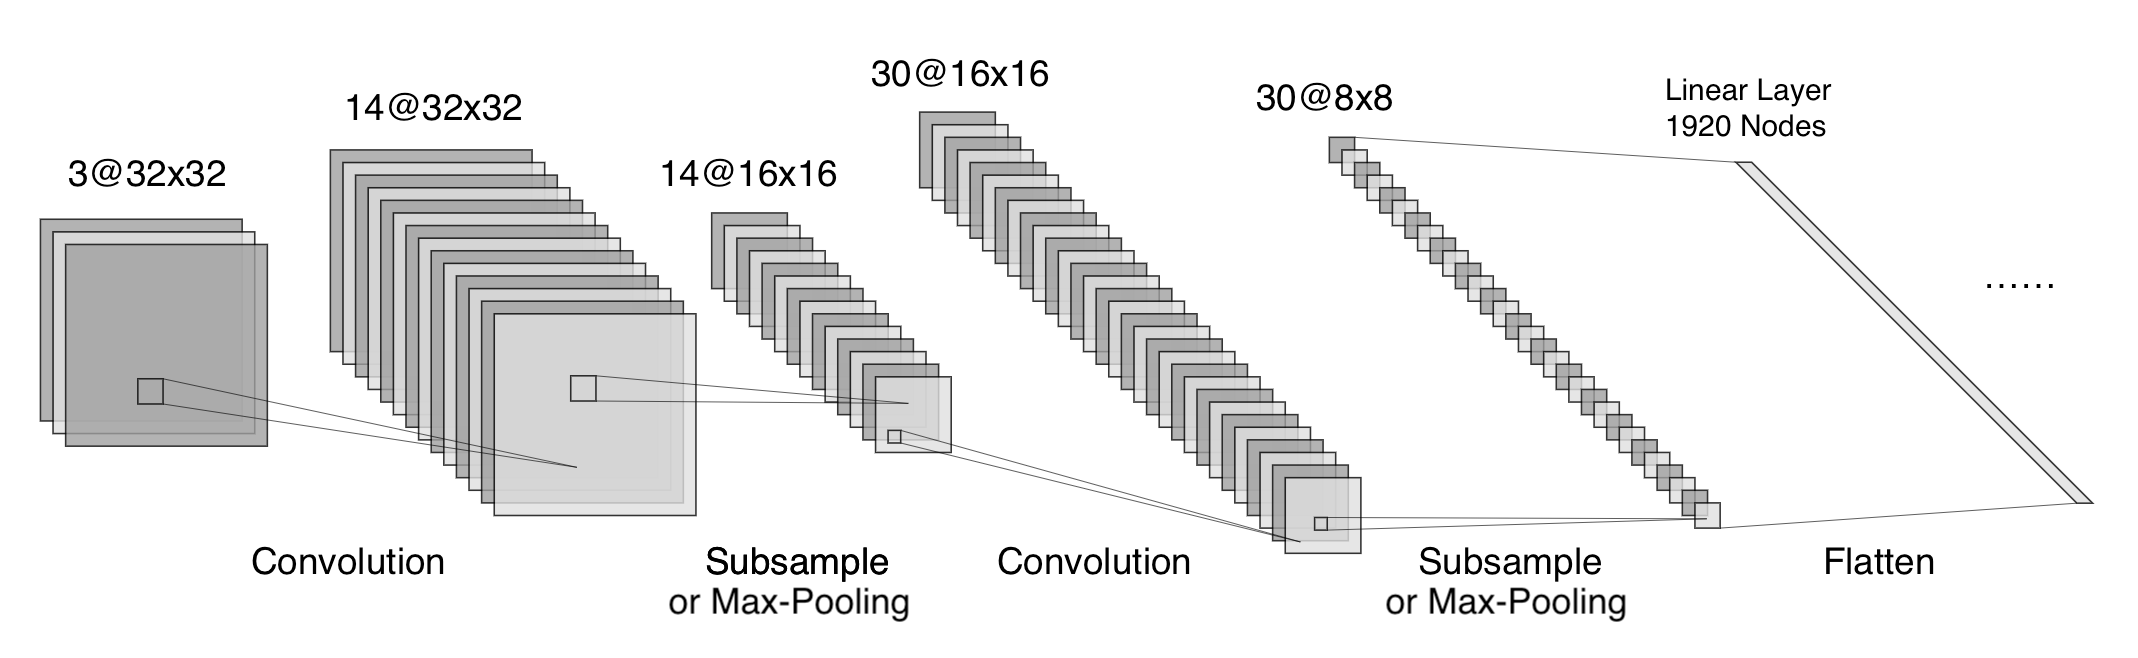
\includegraphics[height = 60mm, width=160mm]{imgs/cnn_s1.png}
\caption{Convolution Neural Network Basic Structure}
\label{fig:cnn1}
\end{figure}

Each convolutional layer $\mathbf{h}^{(l)}$ is organized as a series of channels, where each channel is obtained by a kernel, $\mathbf{W}_{i, j}$ operating on the previous layer's $\mathbf{h}^{(l-1)}$ which was also organized as a series of channels.  Each kernel operation is a local weighted sum of the values within each channel. That is, when there are multiple channels, this weighted sum is over the multiple channels. Once the weighted summations have been performed, a bias term is generally added, and a non-linear transformation, such as the ReLU activation function, is applied to the result. For example, consider Figure 3.3. The first layer, $\mathbf{h}^{(0)}$ is the input image with 3 channels (which coresspond to Red, Green, and Blue), and after applying the kernel operations with the bias and ReLU transformation, the subsequent layer, $\mathbf{h}^{(1)}$, increases to 14 channels. 

We may also present the operations of a convolutional layer more formally. Let $\mathbf{x}_{i j} \in \mathbb{R}^{C_{l-1}}$ represent the vector of values at the $(i, j)$th coordinate for each of the $C_{l-1}$ channels in the $(l-1)$th layer, and let $\mathbf{y}_{i j} \in \mathbb{R}^{C_{l}}$ represent the vector of values at the $(i, j)$th coordinate for each of the $C_{l}$ channels in the $l$th layer. The kernel operation is equivalent to the following linear transformation: $$\tilde{\mathbf{x}}_{i j} = \sum_{\Delta i = -k_1}^{k_1} \sum_{\Delta j = -k_2}^{k_2} \mathbf{W}_{\Delta i \text{ } \Delta j} \text{ } \mathbf{x}_{i+\Delta i \text{ } j+\Delta j}$$ where $\mathbf{W}_{\Delta i \Delta j} \in \mathbb{R}^{C^{l} \times C^{l-1}}$ is learned and the kernel dimensions are fixed at $2k_1$ by $2k_2$. As mentioned above, the bias term, $\mathbf{b}_{l}$, is added and the ReLU transformation is applied such that: $$\mathbf{y}_{i j} = \text{ReLU}(\tilde{\mathbf{x}}_{i j} + \mathbf{b}_{l})$$ where $\mathbf{b}_{l}$ is learned and the ReLU transformation is applied element-wise.

For each convolutional layer, a method of \textit{pooling} or \textit{sub-sampling} is generally done after the above transformations are performed. Pooling and sub-sampling methods are performed to effectively downsample the output of the convolutional layer along its spatial dimensions. That is, the size of each channel is reduced. While the convolutional layer of $h^{(l-1)}$ is generally meant to increase the number of channels, the pooling or sub-sampling method is applied to decrease the height and width of each channel. The primary goal of pooling and sub-sampling is to reduce the total number of parameters within the network. Consequently, this reduces the chance of overfitting our training data and significantly increases training time.

As mentioned previously, we trained a total of two multi-network ensembles. The first ensemble includes a standard CNN for the image data and a multi-layer perceptron for the patient-level metadata, while the second ensemble includes a ResNeSt network for the image data and a similar multi-layer perceptron for the patient-level metadata. The first ensemble was used as a model to compare the ResNeSt model with. It can be thought of as a baseline model to assess the improvements provided by the split-attention networks within the second ensemble. 

The CNN within the first ensemble contained a total of 6 convolutional layers. Each convolutional layer was immediately followed by batch-normalization and downsampling. The convolutional layer within this ensembles exclusively applied \textit{max-pooling} as its downsampling method. For each channel, max-pooling simply replaces the value of each pixel by the maximum of a fixed-size patch surrounding the pixel. In this case, we decided to use max-pooling with a kernel size of $2 \times 2$ and a stride of 2. Figure 3.4 demonstrates a simple example of how max-pooling is applied to the spatial data within each channel. 

\begin{figure}[h]
\centering
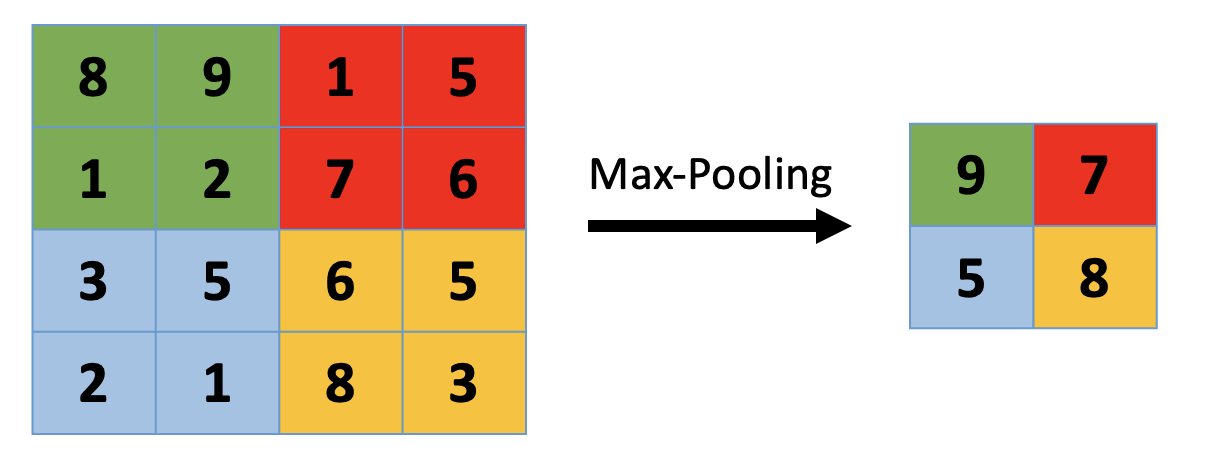
\includegraphics[height = 30mm, width= 80mm]{imgs/maxpool.png}
\caption{Max-Pooling Example with Filter-Size $2 \times 2$ and Stride 2}
\label{fig:maxpool}
\end{figure}

\begin{table}[h!]
\centering
\footnotesize 
\renewcommand{\arraystretch}{1.3}
\begin{tabular}{ c | c | c | c | c | c | c} 
\hline
\makecell{\textbf{Layer} \\ \textbf{Name}} & \makecell{\textbf{Output} \\ \textbf{Size}} & \textbf{Operation} & \makecell{\textbf{Output} \\ \textbf{Channel} \\ \textbf{Number}} & \textbf{Normalization} & \textbf{Activation} & \textbf{Pooling}\\ 
\hline
\hline
Conv1 & 253x253 & $7 \times 7$ & 6 & \makecell{Batch-Norm \\ (2D)} & ReLU & \makecell{Max-Pool \\ (2x2, stride=2)}\\
\hline
Conv2 & 124x124 & $7 \times 7$ & 15 & \makecell{Batch-Norm \\ (2D)} & ReLU & \makecell{Max-Pool \\ (2x2, stride=2)}\\
\hline
Conv3 & 59x59 & $7 \times 7$ & 30 & \makecell{Batch-Norm \\ (2D)} & ReLU & \makecell{Max-Pool \\ (2x2, stride=2)}\\
\hline
Conv4 & 26x26 & $5 \times 5$ & 60 & \makecell{Batch-Norm \\ (2D)} & ReLU & \makecell{Max-Pool \\ (2x2, stride=2)}\\
\hline
Conv5 & 11x11 & $5 \times 5$ & 80 & \makecell{Batch-Norm \\ (2D)} & ReLU & \makecell{Max-Pool \\ (2x2, stride=2)}\\
\hline
Conv6 & 3x3 & $3 \times 3$ & 100 & \makecell{Batch-Norm \\ (2D)} & ReLU & \makecell{Max-Pool \\ (2x2, stride=2)}\\
\hline
Linear1 & 1x1 & Fully Connected & 512 & \makecell{Batch-Norm \\ (1D)} & ReLU & N/A\\
\hline
Linear2 & 1x1 & Fully Connected & 512 & \makecell{Batch-Norm \\ (1D)} & ReLU & N/A\\
\hline  
\end{tabular}
\label{tab:CNN_arch}
\caption{CNN Architecture for Multi-Network Ensemble \#1}
\end{table}

After all 6 convolutional, normalization, and downsampling operations are applied, the original 3-channel image is filtered to a linear layer with exactly 900 nodes. As described above, this output should respresent the high-level features within the images. We include two additional fully-connected layers, each with 512 nodes, in another attempt to learn any remaining non-linear combinations of these features. Note that all convolutional and linear layers associated with this network used the ReLU activation function. Table 3.1 includes the details regarding the specific architecture used for the CNN within our first ensemble.

In parallel to this convolutional network, the multi-layer perceptron takes the 7 patient-level features (after one-hot encoding) and connects it to a linear layer with 256 nodes. A batch-normalization layer is also included, and dropout regularization with $p=0.2$ is used to prevent overfitting. Again, we note that the ReLU activation function was used for this multi-layer perceptron. 

\begin{figure}[h]
\centering
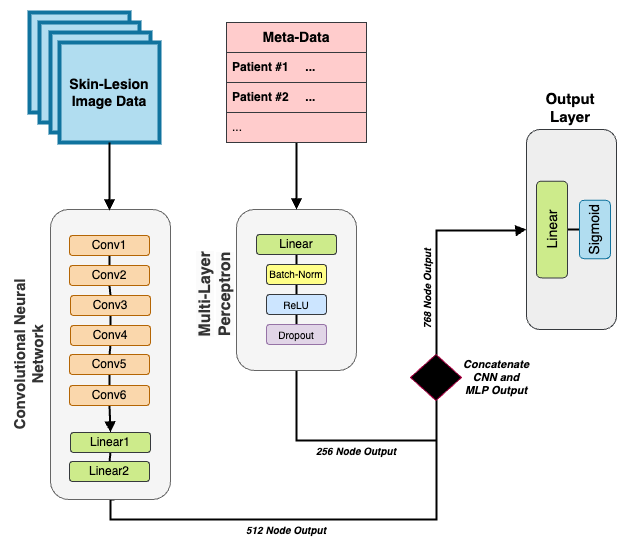
\includegraphics[height = 100mm, width= 120mm]{imgs/ens1_arch.png}
\caption{Multi-Network Ensemble \#1}
\label{fig:ens1_arch}
\end{figure}

Figure 3.5 illustrates how these two seperate networks are effectively fused together for our first ensemble. The 512 node output corresponding to the image-data CNN is concatenated with the 256 node output corresponding to the patient-level metadata. This concatenated layer is then fed into the output layer, with a single node. Lastly, we applied the sigmoid function to the score of the output node in order to estimate the probability that the associated skin-lesion is malignant.

The framework of this first multi-network ensemble is very similar to the framework used in the second ensemble. In the next section, we first discuss the ResNeSt network itself, and how it can be used to better extract the high-level features within the skin-lesion images. Then, we provide the details regarding how it was used within our second multi-network ensemble.

\subsection{ResNeSt}

Write about evolution from CNN to ResNet to ResNeSt. Also use the following description of ResNeSt somewhere (from pytorch website):

While image classification models have recently continued to advance, most downstream applications such as object detection and semantic segmentation still employ ResNet variants as the backbone network due to their simple and modular structure. We present a simple and modular Split-Attention block that enables attention across feature-map groups. By stacking these Split-Attention blocks ResNet-style, we obtain a new ResNet variant which we call ResNeSt. Our network preserves the overall ResNet structure to be used in downstream tasks straightforwardly without introducing additional computational costs. ResNeSt models outperform other networks with similar model complexities, and also help downstream tasks including object detection, instance segmentation and semantic segmentation.

A New ResNet Variant, is modularized architecture is designed to apply the channel-wise attention on different network branchesresidual-network variant known as \textit{ResNeSt}.

Disuss the use of the mentioned Image Augmentations and then discuss the idea of Batch Normalization, Adam Optimizer, L2 Regularization, and Dropout layers. Discuss the difference between starting the CNN weights at random values, vs starting the ResNeSt weights at the IMAGENET trained weights and finetuned for our set of data (effectively leveraging their training).

However, with average-pooling, the value of each pixel, for each channel, is replaced with the average of the patch surrounding the pixel. The convolutional layers within our ensemble that uses the ResNeSt network exclusively uses average-pooling with a kernel size of $3 \times 3$ or $2 \times 2$ depending on the location of the layer within the network. However, 

\subsection{Network for Patient-Level Features}


One dropout layer was included in the final fully-connected layer of our convolution network and another dropout layer was included in the multi-layer perceptron for the 

%%%%%%%%%%%%%%%%%%%%%%%%%%%%%%%%%%%%%%%%%%%%%%%%%%%%%%%%%%%%%%%%%%%%%%%%

\chapter{Results}

% if time, use import tikzplotlib

\section{CNN + MLP Ensemble Results}

Write here. Give all plots from analysis notebook. Give table of statistics and confusion matrix.

\section{ResNeSt + MLP Ensemble Results}

Write here. Write here. Give all plots from analysis notebook. Give table of statistics and confusion matrix. Compare to regular CNN + MLP model.

%%%%%%%%%%%%%%%%%%%%%%%%%%%%%%%%%%%%%%%%%%%%%%%%%%%%%%%%%%%%%%%%%%%%%%%%

\chapter{Conclusion and Future Work}

Write here.

%%%%%%%%%%%%%%%%%%%%%%%%%%%%%%%%%%%%%%%%%%%%%%%%%%%%%%%%%%%%%%%%%%%%%%%%

\bibliography{bib/resnest_melanoma_detection.bib}    % bibliography references
\bibliographystyle{uclathes}


\end{document}